\subsection{Calibration}\label{calibration}
The model parameters were calibrated to match the prevalence across the ongoing Malawian epidemic. Note that there is no particular convention to identify in the data, any of the four theoretical stages described in the model. For example the \textit{pre-epidemic stage} does not exist in real life, so there is no way to assign values to it. In addition the model does not discriminate between male and female individuals; disaggregation that is important when characterizing the education gradient by gender.\\

For calibration purposes I make an assumption regarding the gender of the individuals. I assign the role of sex buyers to men and sex producers to women. As described in Section\ref{sec1} there is no convention that prevents the types to be classified in the opposite way. From now on I will refer to type one individuals as men and type two as women. As it will be shows this assumption does not affect the main results of the paper.\\

  I use data from 2000 for the calibration of  the \textit{myopic stage} of the epidemic, I chose 2000 since the Malawian HIV/AIDS epidemic reached a peak around that year. The HIV prevalence in Malawi in 2000 reached 16.8 percent of the total population, and this is the number I will be targeting. Unfortunately there is no additional data concerning the prevalence across educational groups by gender in 2000, so it is not possible to calibrate this numbers to values found in the data. However using linear interpolation methods by taking the prevalence values for 2004 as a reference, the estimated HIV prevalence for educated females reaches 19.3 percent in 2000, I therefore use this value as a benchmark to calibrate the endogenous prevalence for educated females that the model  generates. \footnote{Again, there is no particular reason other than the calculation of the HIV education gradient, for which I choose to match these prevalences .}\\
  
 The \textit{maturity and diffusion} of the epidemic is calibrated to match the prevalence of the year 2004, in addition the actual value of the HIV prevalence rate among educated females and males will be used for the calibration.  Finally, I use the data for 2010 to calibrate the \textit{ART's stage} of the epidemic . Although antiretroviral treatment was introduced in Malawi in the year 2005, the effects are visible 5-6 years after, then it is reasonable to think 2010 as the last stage of the epidemic described by the model.  Table\ref{tablefinal1} through Table\ref{tablefinal3} show the parameters inherent of each stage of the Malawian HIV/AIDS epidemic. The rest of the parameters which I assume are not stage specific are summarized in \ref{tablefinal4}: 
\begin{table}[H]
\centering
\caption{Targeted Prevalences (in $\%$) }
\label{tablefinal1}
\begin{tabular}{c|>{\centering\arraybackslash}m{0.7cm}|>{\centering\arraybackslash}m{2cm}|c|c}
\hline
\multirow{2}{*}{\textbf{Stage}}& \multirow{2}{*}{\textbf{Year}} &  \multirow{2}{*}{\textbf{Total}}&  \multicolumn{2}{|>{\centering\arraybackslash}m{4cm}}{\textbf{HIV/AIDS Prevalence of (*) who completed higher education or more}}\\
\cline{4-5}
&&&(*)\textbf{Females}&(*)\textbf{Males}\\
 \hline \hline
 Myopic Stage& 2000 & 15.0 & 19.3 &16.5\\
 [0.3em]
 Maturity    & 2004 & 11.8 & 15.1 &12.9\\
 [0.3em]
 ARTs        & 2010 & 10.7 & 16.1&8.9\\
\hline \hline
\end{tabular}
\begin{flushleft}
Sources: Taken form DHS data.
\end{flushleft}

\end{table}



\begin{table}[H]
\centering
\caption{Fertility and mortality rates}
\label{tablefinal2}
\begin{tabular}{c|c|>{\centering\arraybackslash}m{2.5cm}|>{\centering\arraybackslash}m{4cm}|>{\centering\arraybackslash}m{4cm}}
\hline
 \textbf{Stage}& \textbf{Year} & \textbf{Fertility rate($\%$)} & \textbf{Mortality rate including HIV/AIDS infected($\%$)}&\textbf{Mortality rate excluding HIV/AIDS infected($\%$)} \\
 \hline \hline
 Myopic Stage& 2000 & 6.20 &1.68&1.35\\
 [0.3em]
 Maturity    & 2004 & 5.95 &1.45&1.04\\
 [0.3em]
 ARTs        & 2010 & 5.30 &0.98&0.71\\
 \hline \hline
\end{tabular}
\begin{flushleft}
Sources:  World Bank, Sustainable Development Indicators.
\end{flushleft}
\end{table}

\begin{table}[H]
\centering
\caption{Share of people educated but infected}
\label{tablefinal3}
\begin{tabular}{c|c|>{\centering\arraybackslash}m{2.2cm}|>{\centering\arraybackslash}m{1.5cm}|>{\centering\arraybackslash}m{2.2cm}|>{\centering\arraybackslash}m{2.2cm}}
\hline
 \multirow{ 2}{*}{\textbf{Stage}}&\multirow{ 2}{*}{\textbf{Year}}&\multicolumn{2}{>{\centering\arraybackslash}m{6cm}}{\textbf{Share of (*) with secondary education or more($\%$)}}&\multicolumn{2}{|>{\centering\arraybackslash}m{6cm}}{\textbf{Share of (**)with secondary education or more and are infected ($\%$).}\vspace{0.1cm}}\\
 [0.6em]
 \cline{3-6}
  &  & \textbf{(*)Females}&\textbf{(*)Males} &\textbf{(**)Females}&\textbf{(**)Males} \\
 \hline \hline
 Myopic Stage& 2000 &11.1&20.9&2.1&3.4\\
 [0.3em]
 Maturity    & 2004  &15.5&27.2&2.3&3.5\\
 [0.3em]
 ARTs        & 2010 &20.0&31.2 &3.2&2.8\\
 \hline \hline
\end{tabular}
\begin{flushleft}
Sources:  DHS data .
\end{flushleft}
\end{table}



\begin{table}[H]
\centering
\caption{Parameters which are not stage specific}
\label{tablefinal4}
\begin{tabular}{c|c|c|c}
\hline
 \textbf{Parameter Symbol}&\textbf{Value}& \textbf{Description} & \textbf{Source}\\
 \hline \hline
 $\mu$& 3.00 & Risk Aversion & Standard value \\
 [0.3em]
 $\beta$& 0.96 & Subjective discount factor & Standard value  \\
 [0.3em]
 $\alpha$& 0.1& Labor income share  & - \\
 [0.3em]
 \hline \hline
\end{tabular}
\begin{flushleft}
\end{flushleft}
\end{table}
\section{Results}\label{sec6}
Once the model was calibrated in each stage  respectively, the value functions an policy functions were approximated via value function iteration. Figure\ref{lafigura1} to Figure\ref{lafigura7} show the obtained value functions, and the policy functions for asset holdings, consumption and extra-marital risky sex consumption, by type of agent in each stage of the epidemic. Starting from stage 1 we can see that educated individuals hold a larger amount of assets than the less educated individuals, regardless of their type. Also from stage 2 we see that educated individuals who are not infected are wealthier, consume more and incur in more extra-marital risky sex than the less educated counterparts. Note that the effect is reversed when looking at sex producers. As expected, the policy function for sex production is flat, since the individual supplies a constant account of labor to the sex market.\\

A key result of the model is the endogenous reduction of extra-marital sex consumption once the risk for HIV infection is acknowledged. We can see this phenomenon by comparing Figures \ref{stage_2fig_1},\ref{stage_2fig_2} with Figures \ref{stage_4fig_1},\ref{stage_4fig_1}. These figures show the extra-marital risky sex consumption policy function for Stage 2 and Stage 3 respectively, it is clear than individuals realize that the chances of infection increase with the amount of extra-marital risky sex consumed, then they automatically decide to reduce the amount consumed. \\

Without the need to run simulations, we can take the data provided by the model and calculate the education gradient for the total Malawian population and its dis-aggregation by gender. The model outputs data in a panel structure. Since the model assumes a continuum of individuals I choose to generate a sample of size $N=20000$. Only in this sense is this data more convenient than  survey data. However, Survey data is richer in all senses, as it allow us to control for other aspects that the model cannot simulate. The data used to calculate the educational gradient includes:  HIV prevalence of the whole population, and the portion of the population who is educated but infected, and its respective gender equivalents. \\  

\subsection{A linear probability model}
Following \cite{raul}, I propose a linear probability model with the HIV status of the individual across stages as dependent variable and the level of education as an independent variable.\\

Consider the panel structure generated by the model $X_{i,t}$ where $y_{i,t}, s_{i,t}\in X_{i,t}$. Where $i$ indexes the individuals $i\in \{1,...,N\}$ and $t$ indexes the stage of the epidemic $t\in \{2,3,4\}$\footnote{Note that $t$ starts in Stage 2, since as explained in Section\ref{calibration} Stage 1 does not exist in real life}. Here $y_{i,t}$ denotes the HIV status of an individual $i$ living in stage of the epidemic $t$; $edu_{i,t}$ denotes the education status of the individual $i$ in stage $t$. Then the linear projection of $y$ on $s$ is:
\begin{align}
y_{i,t}=\alpha_{2}+\sum_{t>2}\alpha_{t}\mathbf{1}_{t}+(\gamma_{2}+\sum_{t>2}\gamma_{t}\mathbf{1}_{t})edu_{i,t}+\epsilon_{i,t}
\end{align}
 $\mathbf{1}_{t}$ is the indicator function that takes the value of $1$ if we are in epidemic stage $t$ otherwise is zero. Given the structure of the model we can be sure that $E(\epsilon)=0$ and $Var(\epsilon)=\sigma^{2}$, then the model can be estimated via OLS.\\
 
 Keep in mind that in this model $y_{i,t}$ and $s_{i,t}$ are both categorical variables since the model only distinguishes between the individuals who finished secondary education and the ones who didn't. Given this, the calculation of the gradient differs from the conventional one. In this model the base category $\alpha_{2}$ represents those individuals who are in the \textit{myopic stage} and have not finished secondary education. $\gamma_{2}$ is the HIV-education gradient in the \textit{myopic stage} of the epidemic. In the same way $\gamma_{2}+\alpha_{t}+\gamma_{t}$ is the HIV-education gradient in stage $t$, then the difference in the HIV education gradient between an individual in stage $t$ and the \textit{myopic stage} is $\alpha_{t}+\gamma_{t}$. The interpretation of the HIV-economic gradient is as follows; in the\textit{myopic stage}, finishing secondary education or getting higher levels of education changes the probability of being infected by $\gamma_{2}$ percent. In later stages, the probability of of being infected changes by $\gamma_{2}+\alpha_{t}+\gamma_{t}$ percent.\\
 
  Table\ref{gradient} shows the results of the linear probability model. This includes the models for the total population, and the dis-aggregation by gender. 
\begin{table}[H]
\centering
  \caption{The HIV-education gradient for Malawi} 
  \label{gradient} 
{
\def\sym#1{\ifmmode^{#1}\else\(^{#1}\)\fi}
\begin{tabular}{l c c c}
\hline\hline\\[-1.8ex] 
 & \multicolumn{3}{c}{\textit{Dependent variable: HIV Status}} \\ 
\cline{2-4}\\[-1.8ex]  
            &\multicolumn{1}{c}{Total population}&\multicolumn{1}{c}{Males}&\multicolumn{1}{c}{Females}\\
   %         &\multicolumn{1}{c}{OLS}&\multicolumn{1}{c}{OLS}&\multicolumn{1}{c}{Logit}&\multicolumn{1}{c}{Logit}\\
\hline\\[-1.8ex] 
Education      &      0.0290\sym{***}&      0.0441\sym{***}&     0.0242\sym{***}  \\
            &    (0.0000)         &    (0.0000)         &     (0.0000)   \\
[0.25em]
Stage 3     &     -0.0324\sym{***}&     -0.0277\sym{***}  &   -0.0392\sym{***} \\
            &    (0.0000)         &    (0.0000)         &     (0.0000)   \\
[0.25em]
Stage 4 &     -0.0431\sym{***}     &     -0.0423\sym{***}       &       -0.0479\sym{***}\\
    &    (0.0000)         &    (0.0000)         &     (0.0000) \\
[0.25em]
Education *Stage 3    &      -0.0111\sym{***}&      -0.0225\sym{***} &      -0.0030\sym{***} \\
            &    (0.0000)         &    (0.0000)         &     (0.0000)  \\
            [0.25em]
Education *Stage 4 &     -0.0174\sym{***}&     -0.0358\sym{***}&      0.0158\sym{***} \\
            &    (0.0000)         &    (0.0000)         &     (0.0000)  \\
[0.25em]
            
\hline\\[-1.8ex] 
            
Intercept      &      0.1496&      0.1237&      0.1689\\
            
\hline\\[-1.8ex] 

\(N\)       &        20000         &        10000 &        10000   \\
\hline\hline\\[-1.8ex] 
\multicolumn{4}{l}{\footnotesize Standard errors in parentheses. Two-tailed test.}\\
\multicolumn{4}{l}{\footnotesize \sym{*} \(p<0.1\), \sym{**} \(p<0.05\), \sym{***} \(p<0.01\)}\\
\end{tabular}
}
\end{table}

The results in Table\ref{gradient}are in line with the findings by \cite{raul}. The HIV educational gradient in the myopic stage of the epidemic is significantly positive, both in the total population as well as the gender dis aggregation. The rest of the coefficients are significantly negative, meaning that in later stages of the epidemic, additional education represents a reduction of the probability of infection. The HIV education gradient by stage of the epidemic is summarized in Table\ref{gredient} and graphed in Figure\ref{fig_grad1} and Figure\ref{fig_grad2}.

 \begin{table}[H]
 \centering
 \caption{HIV-education gradient by stage of the epidemic and by gender($\%$)}
\label{gredient}
\begin{tabular}{>{\arraybackslash}m{6cm}|c|c|c}
\hline
 \textbf{HIV-Education Gradient}& \textbf{Total} & \textbf{Males}& \textbf{Females} \\
 \hline\hline
 \textit{Myopic stage}($\gamma_{2}$)& $2.9$ & $4.41$& $2.42$\\
 [0.25em]
 \textit{Maturity stage}($\gamma_{2}+\alpha_{3}+\gamma{3}$)&$-1.45$ & $-0.60$& $-1.80$ 
 \\ 
 [0.25em]
 \textit{ARTs stage}($\gamma_{2}+\alpha_{4}+\gamma{4}$)
 & $-3.16$& $-3.39$& $-0.79$\\
 \hline\hline
\end{tabular}
\end{table}

The results in Table\ref{gredient} can be interpreted as follows. In the \textit{myopic stage} people who finish secondary education or have more years of education, increase their probability of getting HIV infected by 2.9$\%$. However on later stages of the epidemic, namely the \textit{myopic stage} and the \textit{maturity stage}, increasing years of education beyond secondary education reduces the chances of HIV infection by 1.45$\%$ and 3.16$\%$ respectively. When looking at the gender dis-aggregation, we can see that education beyond secondary increases the probability of HIV infection in the \textit{myopic stage} by 4.41$\%$ but in the \textit{ARTs stage}, additional education, reduces the risk oh HIV infection by 3.39$\%$. The same occurs in the case of females, but the reduction is however the probability of infection does not reduce as much as in the two other cases.\\

Figure\ref{fig_grad1} shows that the educational gradient is concave up, and starts to have the U shape described by \cite{raul}. Nevertheless, in Malawi the HIV-education gradient starts positive in the early stages, but turns significantly negative in the last two stages. This suggest that it is wise to encourage education in the latest stages of the epidemic, as this will reduce the probabilities of infection in the future.\\

 The HIV education gradient for females has a clear U shape. The gradient start at $2.42$ $\%$ during the \textit{myopic stage} but then turns negative  to rise again after reaching its lower value in the during the \textit{maturity stage} . This means that educated women in the latest stages should be considered as a vulnerable target group. When looking at the gradient of men, we see that it has a clear downward sloping shape. More precisely, additional years of education for men will reduce their chances of HIV infection. Then, targeted intervention should include all those individuals  who possess less education.  We can also see that the HIV gradient for females is larger in magnitude than that of men. In neither of the cases the gradient turns to positive during the \textit{ARTs stage} . This a big difference when comparing with the results obtained for Sub-Saharan Africa. \footnote{See Figure\ref{bild1} to Figure\ref{bild2} in the Appendix\ref{appendix}}
 

\begin{figure}[H]
\centering
\begin{minipage}{.5\textwidth}
 \centering
 \captionof{figure}{HIV-education gradient\\ total}
%\begin{tabular}{l}
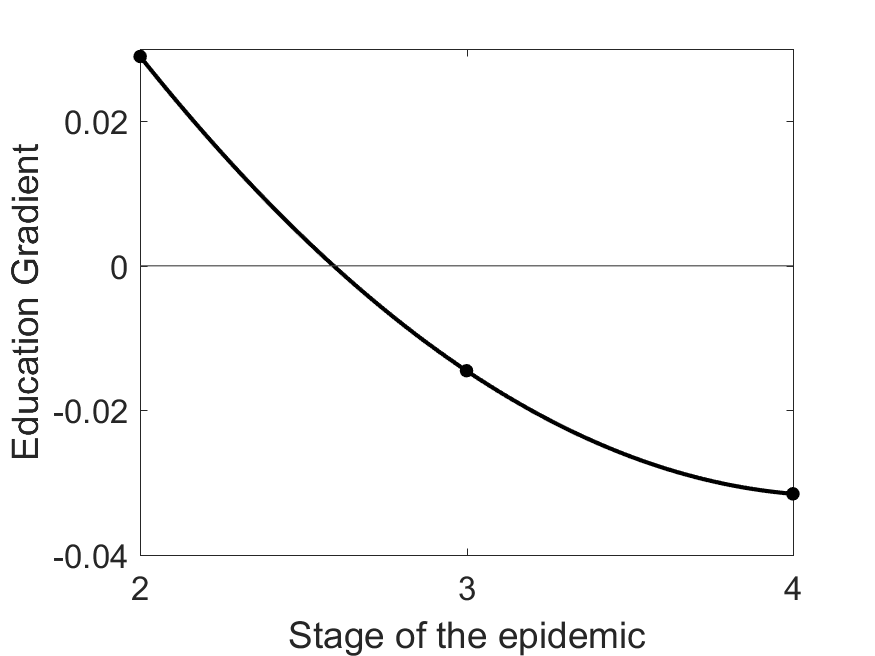
\includegraphics[width = 1\linewidth, height = 0.25\textheight]{figures/gradient/fig_grad1.png}
\label{fig_grad1}
\end{minipage}%
\begin{minipage}{.5\textwidth}
\centering
\captionof{figure}{HIV-education gradient\\ by gender}
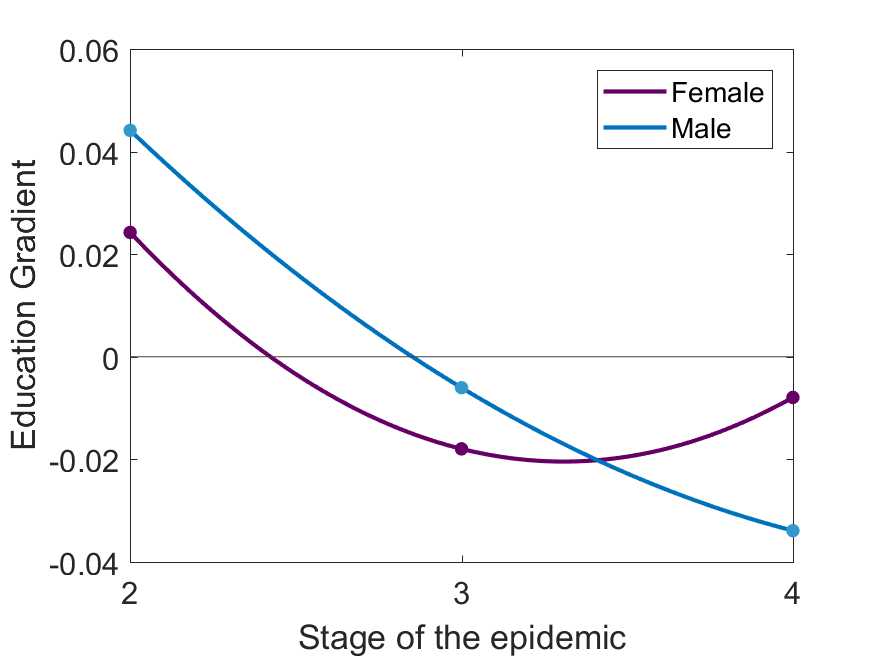
\includegraphics[width = 1\linewidth, height = 0.25\textheight]{figures/gradient/fig_grad2.png}
\label{fig_grad2}
\end{minipage}
\end{figure}

In order to understand the differences between educated risky sex buyers and risky sex producers, it is possible to conduct a simple sensitivity analysis on the estimation results. One way to increase the overall prevalence in the country is to increase labor income given to all individuals, in particular, any individual regardless if she/he is infected or not, will increase its chosen level of extramarital risky sex no matter what because of the income effect, as a result, overall prevalence among the population will increase. A second channel that increases prevalence among the educated buyers or producers is a reduction of the "comprehension parameter" $\rho_{e}$, since educated agents are less aware then they consume more risky sex. However these channels don't tell us anything about the prevalence by gender. On the other hand, there is a set endogenous outcomes generated by the sex market behavior and the amount of risky sex demanded by educated/uneducated sex buyers. In principle, if the price of risky sex increases, the total demand will decrease, how ever total demand might is still covered be covered in the same proportion by educated/uneducated risky sex producers. If demand for risky sex among uneducated sex buyers increases, it might be the case that prevalence among educated women increases since they also have to cover the increasing demand. In other words the market protects educated sex buyers, since in no way they will be forced to increase their sex consumption, but if uneducated buyers increase demand, both uneducated and educated producers must intervene to clear the sex market.    